\graphicspath{{./Annexe_amidon/images/}}

\chapter{Propriétés physico-chimiques de l'amidon}
\label{annexe:amidon}

L'amidon étant un élément naturel, il ne fait pas exception au fait qu'il possède des propriétés structurales complexes, qui engendre évidemment une compréhension assez difficile de ses propriétés physico-chimiques. L'amidon est un élément que l'on trouve dans de nombreux produits issus du règne végétal. On le retrouve notamment dans les céréales et les légumes. Il est généralement extrait et stocké sous forme de poudre fine (grains de 10 à \SI{100}{\micro\meter} selon la variété botanique). Son utilisation est très courante dans les secteurs de l'agroalimentaire, de la papeterie et dans le secteur pharmaceutique. L'amidon est, par exemple, utilisé dans la conception de comprimés pharmaceutiques afin de stocker les principes actifs et ses propriétés chimiques font que la salive peut le transformer en sucre. Il sert donc également en tant qu'activant chimique. Il est utilisé en papeterie afin d'améliorer la résistance au pliage des papiers, et les propriétés d'impression et est utilisé en tant qu'agent de couchage. Dans le secteur agroalimentaire, l'amidon est utilisé en tant qu'épaississant (pour potages et sauces par exemple), pour le coffrage ou capsulage (il sert à coller les capsules de bouteille par exemple) ou comme gélifiant et stabilisant (grande rétention d'eau).
\section*{Composition des grains}
	Il n'existe pas une structure unique du grain d'amidon. chaque grain est différent des autres. Ses propriétés varient en fonction de sa provenance et de sa croissance. Un amidon de pomme de terre n'aura par exemple pas la même structure et les mêmes propriétés qu'un amidon de maïs.
	\begin{figure}\begin{center}
			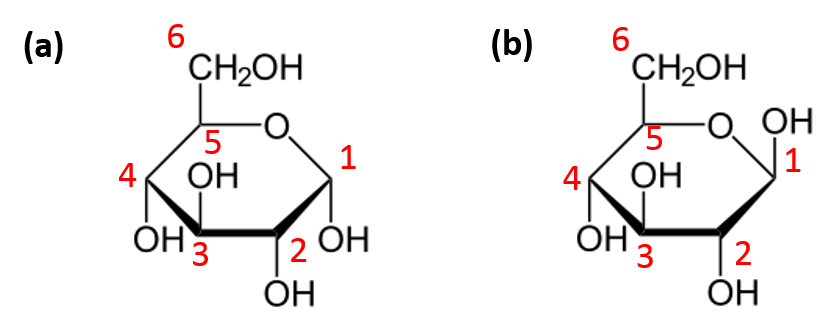
\includegraphics[width=0.5\textwidth]{D-glucose.png}
			\caption{\label{fig03:D-glucose}Les deux isomères majoritaires du D-glucose : (a) $\alpha$-D-glucopyranose et (b) $\beta$-D-glucopyranose}
	\end{center}\end{figure}
	\\A l'échelle moléculaire, l'amidon est constitué d'un assemblage de chaînes moléculaires de D-glucose, de formule $C_6H_{12}O_6$ présenté sur la figure \ref{fig03:D-glucose}. Il s'agit d'un sucre qui peut avoir différentes formes (isomères) : le $\alpha$-D-glucopyranose (présent à 35\% environ) et le $\beta$-D-glucopyranose (65\%). Les chiffres représentés en rouge correspondent aux numéros d'appellation des différentes branches rattachées aux atomes de carbone présents. L'assemblage de ces unités de monomères se fait par l'intermédiaire de liaisons chimiques. Ces liaisons chimiques sont notées de la manière suivante : $$ \text{Type de conformation }\alpha\text{ ou }\beta\ -\left(\text{numéro première branche},\text{numéro seconde branche}\right) $$
	L'amidon est en réalité constitué de deux polymères différents : l'amylopectine et l'amylose. Ces deux homopolymères (puisqu'ils sont tous deux issus du même monomère, le D-glucose) diffèrent selon leur degré de polymérisation et le nombre de ramifications. Leur proportion dans le grain varie en fonction de l'origine botanique (cf. tableau \ref{tab03:difference_grains}).
	\subsection*{Amylose}
		\begin{figure}\begin{center}
				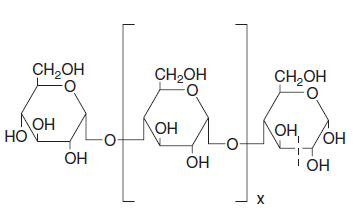
\includegraphics[width=0.4\textwidth]{amylose.png}
				\caption{\label{fig03:amylose}Chaîne moléculaire type de l'amylose}
		\end{center}\end{figure}
		L'amylose est une macromolécule linéaire constituée d'unités de D-glucose rassemblées par les liaisons $\alpha(1,4)$ comme le montre la figure \ref{fig03:amylose}. Le degré de polymérisation de l'amylose atteint généralement 600 et la masse molaire est comprise entre $10^5$ et \SI{e6}{\gram\per\mole}. Il s'agit d'une entité ne présentant pas de ramification.
	\subsection*{Amylopectine}
		\begin{figure}\centering
			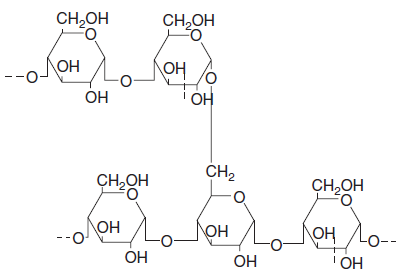
\includegraphics[width=0.4\textwidth]{amylopectine.png}
			\caption{\label{fig03:amylopectine}Chaîne moléculaire type de l'amylopectine}
		\end{figure}
		La figure \ref{fig03:amylopectine} montre l'aspect ramifié de la chaîne moléculaire d'amylopectine. La chaîne est plus courte que celle de l'amylose puisqu'on observe un degré de polymérisation beaucoup plus bas (entre 10 et 60). Les liaisons entre les unités de monomères se font également par la liaison $\alpha(1,4)$ mais peuvent également se faire par liaison $\alpha(1,6)$, ce qui explique les ramifications de la chaîne.
\section*{Structure des grains et conformations cristallines}
	Des études sont actuellement en cours pour comprendre la structure des grains d'amidon mais un modèle se distingue \cite{bemiller_starch:_2009}. Il est présenté sur la figure \ref{fig03:structure_multiechelle}.
	\\Lorsque cela est possible, les chaînes glucosiques de l'amidon vont s'aligner deux à deux et s'enrouler de manière à former une double hélice. Ces doubles hélices vont essayer de trouver une position stable l'une par rapport à l'autre tout en tenant compte des autres éléments présents qui sont les molécules d'eau et les lipides. Les réarrangements possibles sont au nombre de deux et sont présentés en bas de la figure \ref{fig03:structure_multiechelle}. Il caractérisent le type d'amidon (amidon de type A ou de type B). Les amidons de type A présentent un réseau monoclinique et comptent quatre molécules d'eau equiréparties entre les doubles hélices dans une maille élémentaire. Ceux de type B montrent un réseau hexagonal avec six molécules d'eau par maille élémentaire, toutes situées au c\oe{}ur de l'hexagone formé par les doubles hélices. Il existe un amidon de type C pour lequel on retrouve les deux conformations au sein du même grain. Dans ce cas, la structure cristalline de type B est observée plutôt au milieu du grain alors que celle de type A l'est plutôt en périphérie. Les lipides en présence jouent un rôle dans la cristallinité de l'amidon puisqu'ils peuvent former des complexes cristallins avec les chaînes glucosiques. On parlera notamment des structures de type A-L et de type V en fonction de l'ordre de longueur des complexes amylo-lipides.
	\\Des analyses à petite échelle peuvent être menée notamment grâce aux rayons X (diffraction) et à la microscopie électronique en transmission. Ces deux outils permettent de comprendre la structure du grain à l'échelle macromoléculaire (cf. figure \ref{fig03:structure_multiechelle}). L'organisation des doubles hélices donne naissance aux nanocristaux qui se multiplient grâce aux ramifications des chaînes d'amylopectine pour former des "grappes". Ces grappes sont en présence de chaînes d'amylose qui sont complètement indépendantes et qui vont se positionner entre les nanocristaux d'amidon avec les lipides et les molécules d'eau.
	\\Les doubles hélices ont une longueur limitée (entre $5$ et \SI{10}{\nano\meter}). C'est pour cette raison que l'on remarque des zones dans lesquelles aucune structure cristalline n'est observable. Ces zones forment des lamelles amorphes et correspondent aux zones de ramifications de l'amylopectine. Cela explique pourquoi le grain possède une structure "en couches radiales" assez complexes. C'est cette structure semi-cristalline radiale qui permet d'observer au microscope optique en lumière polarisée un effet typique de la biréfringence, que l'on appelle la croix de Malte (une croix se forme sur chaque grain lorsqu'on les observe), quel que soit l'angle de polarisation. Ainsi la cristallinité du grain peut être observée directement par la visualisation de ces croix.
	\\L'alternance des lamelles amorphes et cristallines permet la formation de blocs semi-cristallins appelés "blocklets" qui se regroupent eux-mêmes en "couches radiales" que l'on identifie comme des anneaux de croissance. Les anneaux de croissance sont constitués alternativement de gros blocklets pour former des couches à forte cristallinité et de petits blocklets pour former des couches plus amorphes.
	\begin{figure}\centering
		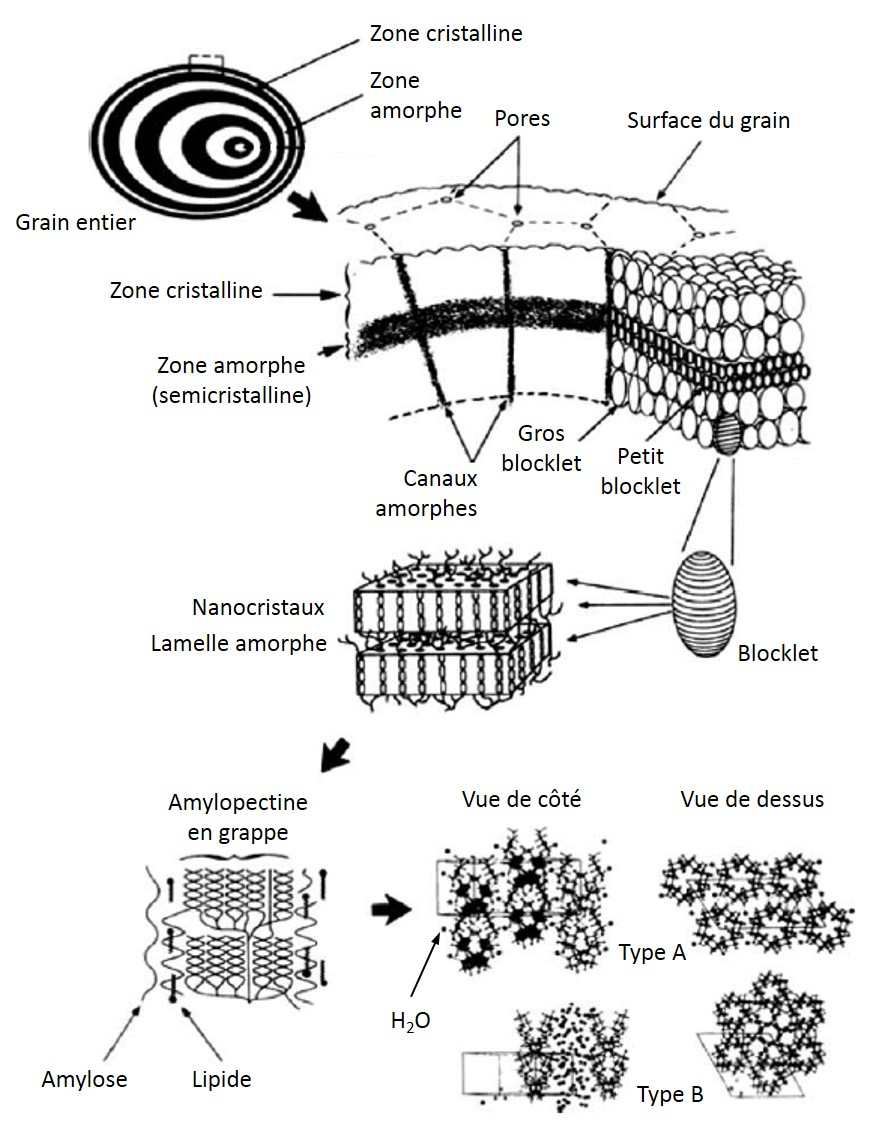
\includegraphics[width=0.7\textwidth]{structure_multiechelle_2.jpg}
		\caption{\label{fig03:structure_multiechelle}Modèle de structure du grain d'amidon à différentes échelles et conformations des macromolécules glucosiques en doubles hélices \citep{bemiller_starch:_2009}}
	\end{figure}
	\\Comme précisé précédemment, le modèle décrit ci-dessus est un modèle type, mais chaque variété d'amidon diffère en fonction de la provenance botanique, de la croissance de la plante, des conditions environnementales, etc. C'est pour cette raison que chaque grain d'amidon d'origine différente est unique. Le tableau \ref{tab03:difference_grains} montre quelques différences observées sur différents types d'amidon.
	\begin{table}\centering
		\begin{tabular}{cccc}
			\hline
			\textbf{Origine botanique} & \textbf{Forme} & \textbf{Taille \si{\micro\meter}} & \% \textbf{Amylose} \\ 
			\hline
			\hline
			Pomme de terre & Ellipsoïdale & 15 - 100 & 23 \\
			Manioc & Hémisphérique, sphérique & 5 - 35 & 17 \\
			Blé & Lenticulaire, polyédrique & 2 - 30 & 26 \\
			Maïs standard & Polyédrique & 5 - 25 & 28 \\
			Maïs cireux & Polyédrique & 5 - 25 & $\leq 1$ \\
			Amylomaïs & Filamenteuse & 5 - 20 & 52 - 80 \\
			Riz & Polyédrique & 3 - 8 & 14 - 32 \\
			Pois lisse & Réniforme & 5 - 10 & 35 \\
			Pois ridé & Rosette & 30 - 40 & 66 \\
			\hline
		\end{tabular}
		\caption{\label{tab03:difference_grains}Propriétés de différents grains d'amidons \citep{bemiller_starch:_2009}}
	\end{table}
\section*{Propriétés physiques et mécaniques}
	\subsection*{Zones amorphes}
		Les propriétés des zones amorphes sont très dépendantes de la température de transition vitreuse. Cette dernière est même, selon \citet{plazek_glass_2007}, le paramètre le plus important pour déterminer les propriétés mécaniques et physiques des polymères amorphes. La transition vitreuse se fait par l'apport d'une énergie calorifique qui permet de rendre les chaînes moléculaires plus mobiles et donc de diminuer la viscosité du matériau. C'est d'ailleurs la raison pour laquelle la mise en forme des polymères se fait au-delà de la température de transition vitreuse, dans un état où la diminution de viscosité permet un écoulement de matière. Cette température dépend des chaînes moléculaires devenant mobiles, mais aussi de paramètres extérieurs tels que la teneur en eau.
		\\En ce qui concerne l'amidon, la température de transition vitreuse est légèrement supérieure à \SI{80}{\celsius} dans les conditions ambiantes. Cependant, la teneur en eau va influencer de manière très importante cette température. En effet, l'eau est un très bon plastifiant pour l'amidon. Une augmentation de la teneur en eau a le même effet sur la mobilité des chaînes qu'une élévation de la température. En fait, l'ajout d'une faible quantité d'eau engendre une augmentation du volume libre et la rupture, ou l'affaiblissement, de certaines liaisons intermoléculaires.
	\subsection*{Zones cristallines}
		Les zones cristallines sont caractérisées par leur température de fusion. Comme l'amidon présente différentes formes de cristallites (double-hélices, complexes amylo-lipides), plusieurs températures de fusion peuvent être déduites d'une courbe de DSC (calorimétrie différentielle à balayage).
		\\Comme pour la transition vitreuse, l'eau a un effet important sur la température de fusion. De la même manière, les molécules d'eau réagissent avec les chaînes ordonnées glucosiques et engendrent une diminution de la température de fusion.
	\subsection*{L'amidon dans son intégralité}
		Il est difficile de caractériser les propriétés mécaniques d'un grain d'amidon puisque la taille moyenne du grain est très petite (entre 2 et \SI{100}{\micro\meter}). Une technique a été mise en place par \citet{willett_mechanical_1994} pour caractériser les grains selon le modèle d'homogénéisation de Halpin-Tsai qui considère un matériau composite dans lequel le renfort est inclus dans la matrice sous forme d'inclusions ovoïdes. Ce modèle est défini selon l'équation (\ref{eq03:Halpin-Tsai}) :
		\begin{equation}\label{eq03:Halpin-Tsai}
		E_c=E_m\left(\frac{1+\xi\eta V_f}{1-\eta V_f}\right), \qquad \eta=\frac{E_f/E_m-1}{E_f/E_m+\xi}\quad\text{et}\quad \xi=\frac{7-5\nu}{8-10\nu}
		\end{equation}
		$E_c$, $E_m$ et $E_f$ correspondent respectivement aux modules de Young du composite, de la matrice et de la fibre. $V_f$ est la fraction volumique en renfort et $\xi$ est un paramètre prenant en compte la géométrie du renfort. La valeur de $\xi$ donnée dans cette équation correspond à la géométrie d'un grain d'amidon issu de pomme de terre, donc de forme ellipsoïdale. Enfin, $\nu$ est le coefficient de Poisson de la matrice considérée.
		\\Afin d'utiliser ce modèle, des grains d'amidon ont été introduits dans une matrice polymère (époxyde et polycaprolactone) dont les propriétés mécaniques sont bien connues. On mesure ensuite le module $E_c$ du composite à l'aide d'un essai de traction puis on remonte, à l'aide du modèle, au module élastique moyen du grain d'amidon. \citet{willett_mechanical_1994} obtient ainsi que le module élastique d'un grain d'amidon de pomme de terre peut atteindre \SI{15}{\giga\pascal}. Cette étude des propriétés mécaniques de l'amidon est cependant un cas isolé puisque d'autres auteurs \citep{schroeter_mechanical_1992, salerno_high_2014} semblent observer des propriétés bien moins bonnes. En effet, la valeur du module élastique - qui est généralement déterminée par microscopie à force atomique (AFM) - varie aux alentours de \SI{2.5}{\giga\pascal}. Cet ordre de grandeur paraît plus cohérent aux vues des valeurs concernant les polymères usuels non orientés. La contrainte maximale en traction serait, quant à elle, située aux alentours de \SI{60}{\mega\pascal}.
		\\Il est également à noter que la géométrie des grains est à prendre en considération. Par exemple, des grains d'amidon de pomme de terre (ellipsoïdaux d'environ \SI{50}{\micro\meter}) ne présenteront pas le même comportement à une sollicitation mécanique que les grains d'amidon de blé (lenticulaires d'environ \SI{15}{\micro\meter}).